\documentclass[nocopyrightspace]{acm_proc_article-sp}
\usepackage{url}
\usepackage{subfig}
\usepackage{color,soul}
\usepackage{enumitem}

\DeclareGraphicsExtensions{.png, .PNG}

\hyphenation{robo-tics amou-nts data-base cho-sen}

\begin{document}
\title{Benchmarking of Relational and NoSQL Databases to Determine Constraints for Querying Robot Execution Logs}
\subtitle{[Final Report]}

\numberofauthors{2} 

\author{
\alignauthor
Alexander J. Fiannaca\\
       \affaddr{Computer Science \& Engineering}\\
       \affaddr{University of Washington}\\
       \email{fiannaca@cs.uw.edu}
\alignauthor
Justin Huang\\
       \affaddr{Computer Science \& Engineering}\\
       \affaddr{University of Washington}\\
       \email{jstn@cs.uw.edu}
}

\date{28 January 2015}

\maketitle

\begin{abstract}
Managing the massive amount of data which flows through the Robot Operating System (ROS) network during operation of a robot is a very challenging task. This has historically been handled by simply storing every message in a flat file (a.k.a. a ROS ``bag file'') which acts as a recording which can later be played back. Unfortunately the rosbag system is not suitable for many useful tasks like querying the messages sent during a certain period to find points in time at which the robot entered or left specific states. In this work, we benchmark several databases with varying storage models in order to determine the best data store for a future application which will subsume the current rosbag system. Our benchmarking study examines the potential throughput of the MongoDb, PostgreSQL, and SQLite3 databases by stress testing each database with workloads that vary the number of messages (rows or documents inserted), the size of messages (size of each insert), and the number of topics (tables or collections being inserted to simultaneously). Additionally, each database is tested against exemplar queries that could be useful for roboticists, and runtimes are reported. Based on these benchmarking studies, recommendations are made for the development of future ROS message logging systems.
\end{abstract}

%\keywords{Databases, Robot Operating System, RDBMS, NoSQL}

\section{Introduction}
\label{intro}

ROS is a popular open-source programming system for robotics, widely used in research circles. In ROS, computation is split across \textit{nodes}, which are processes that may be running across one or more machines. Each node communicates with other nodes through a publisher - subscriber style network by sending messages over named channels called \textit{topics} using typed data structures similar to Google Protocol Buffers. Given a list of topics, messages on these topics can be saved into a custom format, called \textit{bag files}, by a utility called \textit{rosbag}. To analyze the data stored in bag files, the developer must write code to iterate over the recorded data in chronological order. This means that the developer cannot use higher level languages like SQL to transform or query the data. This limitation of bag files has several implications. Primarily these issues surround cases in which researchers want to either find and analyze a subset of the recorded message topics (i.e. only message on the topics base\_odometry/odom and tf), or select messages which meet particular predicates (i.e. messages occurring within five minutes of the robot entering a particular state). In these cases developers must either write one-off scripts to iterate over the messages in the bag file, or use a graphical interface to ``replay'' the messages and manually annotate the times between which they want to gather available messages. Clearly, these approaches are neither reusable or efficient. This problem could be solved if there was a utility that saved the data directly to a database with rich querying capabilities that could allow the developers to more easily access the data of interest through a high level SQL-like data access language.

\begin{figure}
    \centering
    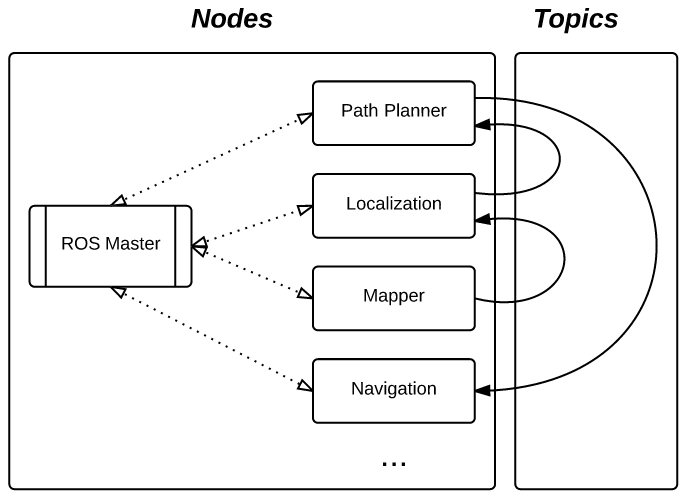
\includegraphics[width=\linewidth]{images/ros}
    \caption{Example of the Architecture of a ROS Network. Nodes are Linux processes which each handle independent tasks. Node communicate by publishing to and subscribing to channels called topics. The master node is a special node in charge of managing topics, publishers, and subscribers.}
    \label{fig:ros}
\end{figure}

In the context of the Robot Operating System, development of a database-backed message logging system is faced with several interesting challenges. First and foremost, the ROS publisher-subscriber network can potentially see data flows on the order of several gigabytes per minute when running a robot such as the PR2. Therefore, an important design decision for this utility would be to ensure the backend data store is capable of persisting large volumes of data in realtime. Additionally, robotics researchers often only have the computer running on the robot (server) and a separate desktop (client) in terms of hardware. Since robotics researchers often do not have a dedicated cluster for storing the data coming off of their robot, the backend data store for this utility needs to be able to provide this high-volume storage while only running on several machines (not a large cluster). Finally, much of the data to be stored consists of numerical values (joint angles, transpose vectors, audio packets, etc) and image-like data (laser scans, point clouds, stereo images, etc.), the data store needs to support rich querying interfaces which make it easy to analyze this type of data. With these considerations in mind, this work evaluates three potential database systems against three main criteria:

\begin{enumerate}
    \item What is the maximum throughput of each database under loads consisting of varying numbers of topics, sizes of messages, and frequency of messages? 
    \item Given a real world bag file dataset (specifically, the MIT Stata dataset), how well does the database perform (e.g. percent of messages persisted) when run in a single machine configuration?
    \item How rich is the query interface supported by the database, and how fast can typical robotics queries be executed? (e.g. ``Select all non-overlapping 1 minute intervals where the robot was in state $X$'', or ``Select all messages beginning 5 minutes before each system error was detected'')
\end{enumerate}

\section{Related Work}
Niemueller et al.~\cite{niemueller2012generic} developed an integration between ROS and MongoDb and benchmarked it. Our experiments use a version of their software, which we improved and modified for the purposes of running our own benchmarks. In their study, they showed that their system was comparable in performance to the native rosbag utility, with improved CPU and memory usage, and 30\% write throughput overhead. However, the paper did not attempt to find the maximum throughput supported by their system. Additionally, they did not compare the performance of their system to that of a relational database. Our work addresses both of these questions.

In a related approach, Dietrich et al.~\cite{dietrich2014ros} developed and benchmarked an integration between ROS and Cassandra, another popular NoSQL database. Their experiments found that their system outperformed a different ROS MongoDb system from the one described above, although the MongoDb system in question was only a data warehouse which stored messages as binary files and therefore had no querying capabilities. In this work, they also did not report the maximum throughput of their system, or do a comparison with relational databases. Importantly, the work of Dietrich et al. was founded on conclusions from a 2012 study by van der Veen et al. \cite{van2012sensor} indicating that Cassandra may be the best database (out of MongoDb, Cassandra, and PostgreSQL) for managing sensor network data. These conclusions in the van der Veen paper rely on a hardware setup of a server with 64 Gb of RAM and 22 CPU cores running their database. While this premise is sound for sensor network data collection, few roboticists have dedicated servers for robot data collection. A far more common setup in a robotics lab is a single external computer, plus the computer on board the robot. Given this stark difference in hardware, the van der Veen work does not appear to be a valid basis for robot data collection systems.

\section{Benchmark Studies}
In order to evaluate these three criteria, we conducted three studies comparing PostgreSQL, MongoDb, and SQLite3: 1) an initial throughput study, 2) a real-world dataset persistence performance study, and 3) a query timing study (corresponding to the three criteria laid out in section \ref{intro}).

\begin{figure}
    \centering
    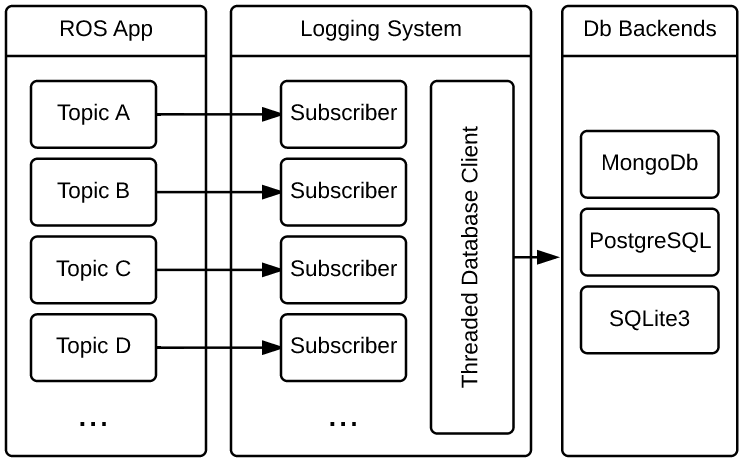
\includegraphics[width=\linewidth]{images/roslog}
    \caption{Design of the ROS Logging Test Framework. The logging system creates a thread for each topic in the current ROS network responsible for converting ROS messages to an equivalent JSON format. The subscriber threads pass prepared JSON messages to a database client responsible for persisting these JSON messages to a particular database.}
    \label{fig:roslog}
\end{figure}

\subsection{Systems and Datasets}
In order to persist ROS messages, all messages were converted to a JSON (Javascript Object Notion) representation. The structure of JSON provides several benefits when it comes to storing ROS messages:
\begin{enumerate}
\item JSON allows for flexibility in message structure, thereby ensuring changes in message structure which are inevitable during the development of a robotics system will not be breaking changes for the datastore,
\item JSON is structured in a very similar manner (nested dictionaries) to that of ROS messages allowing for simple conversion between the formats,
\item JSON can be queried against as opposed to traditional binary message representations.
\end{enumerate}

\begin{figure*}
    \centering
    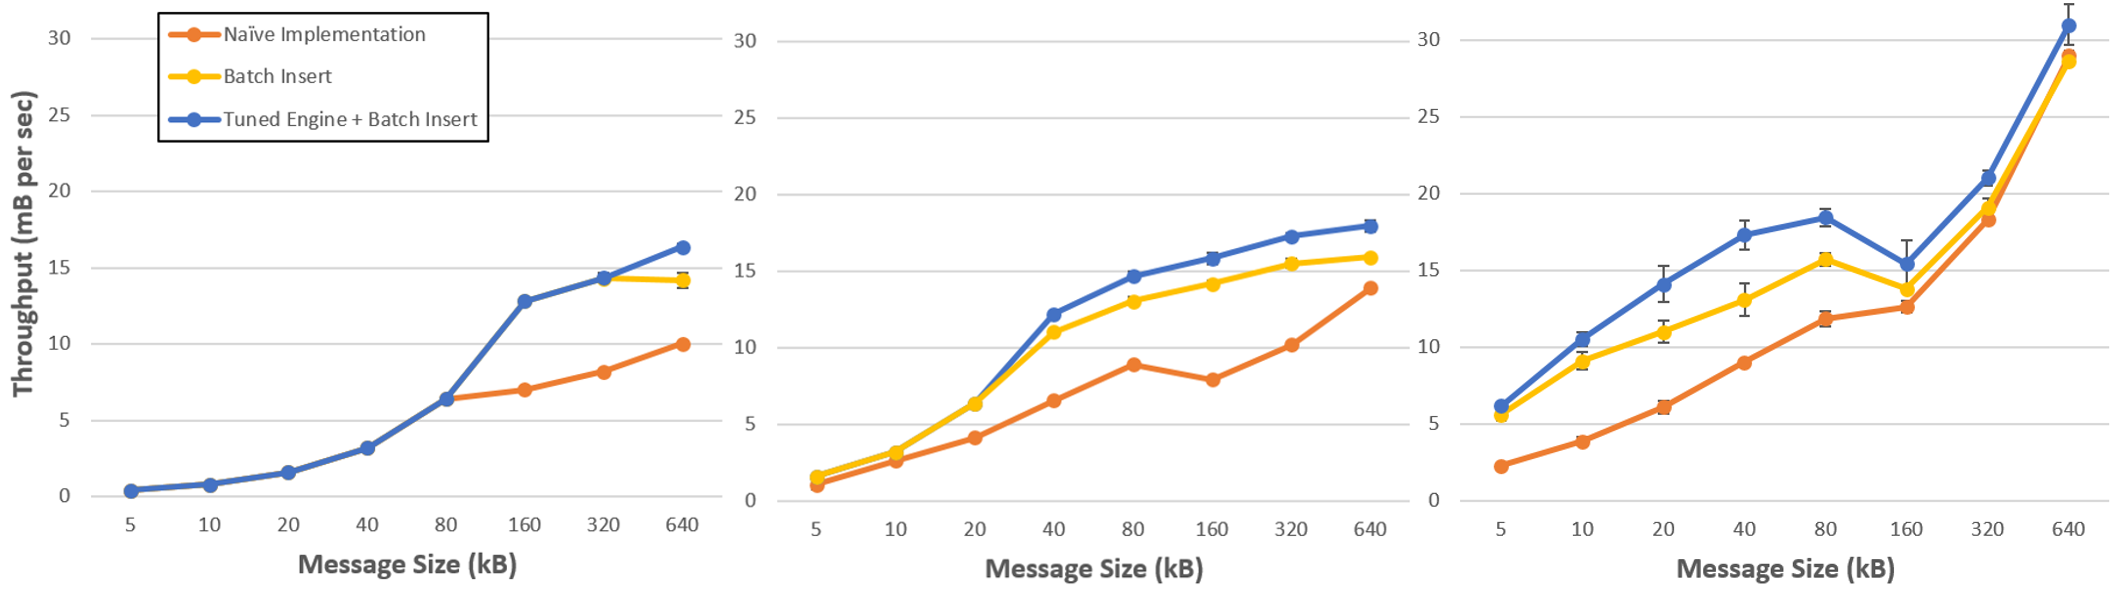
\includegraphics[width=\linewidth]{images/tuning}
    \subfloat[4 Messages Per Second]{%
        \hspace{0.3\linewidth}
        \label{4hz_tuning}%
    }
    \subfloat[16 Messages Per Second]{%
        \hspace{0.4\linewidth}
        \label{16hz_tuning}%
    }
    \subfloat[64 Messages Per Second]{%
        \hspace{0.3\linewidth}
        \label{64hz_tuning}%
    }
    \caption{Tuning PostgreSQL by Testing Throughput Across Multiple Frequencies and Message Sizes}
    \label{fig:tuning}
\end{figure*}

Given this choice of data representation, MongoDb was chosen as a good candidate database for evaluation since MongoDb is a NoSQL document-oriented database which stores all data in JSON and is optimized for fast JSON-based queries. While JSON has not traditionally been considered well suited to being stored in a relational database (having a potentially varied structure), recent advances in PostgreSQL 9.4 have added extensions which allow PostgreSQL to query against JSON data columns in a similar fashion to that of MongoDb, except through the high-level query language SQL. Therefore, PostgreSQL with JSON support was chosen as the second database to evaluate in this study. Finally, initial tests showed that the primary challenge in creating a ROS message logging database is that ROS can have potentially many messages streaming through its network at any given time (on the order of Gb per minute), making it challenging to persist all of the messages in the network as fast as they are generated. For this reason, SQLite3, an embedded database designed to have minimal overhead, was chosen as the third database to evaluate. While future work should be conducted to examine the potential of using streaming engines running on computer clusters for real-time analytics, this work focuses on the more common hardware setup for the average roboticist of a one to two computer system without the requisite resources for running extremely RAM intensive data stores such as the in-memory database VoltDb or the streaming engine Spark Streaming.

For the first criteria evaluated in this study (throughput), a synthetic dataset was generated by creating a message streaming ROS node with the ability to generate multiple topics running at the same frequency and sending messages of the same size in terms of bytes. To test the second criteria (real-world dataset performance), the MIT Stata Center dataset was chosen \cite{fallon2013stata}. This data set encompasses a series of recordings of data from a PR2 robot driving around a building. It includes data types such as laser scans, accelerometer data, and images. While unconventional, these types of data are common in robotics research. The recordings range from 1 - 63 GB in size, representing 1 - 97 minutes in length. Finally, in order to evaluate the third criteria (query performance), built our own data set from a PR2 including message types other than images and laser scans (e.g. joint position messages, audio messages, etc.) which are useful for testing queries against data reflecting a broad subset of possible message types in the ROS environment (\textit{note, this final dataset has yet to be created, and may change before the final submission}).

\begin{figure*}
    \centering
    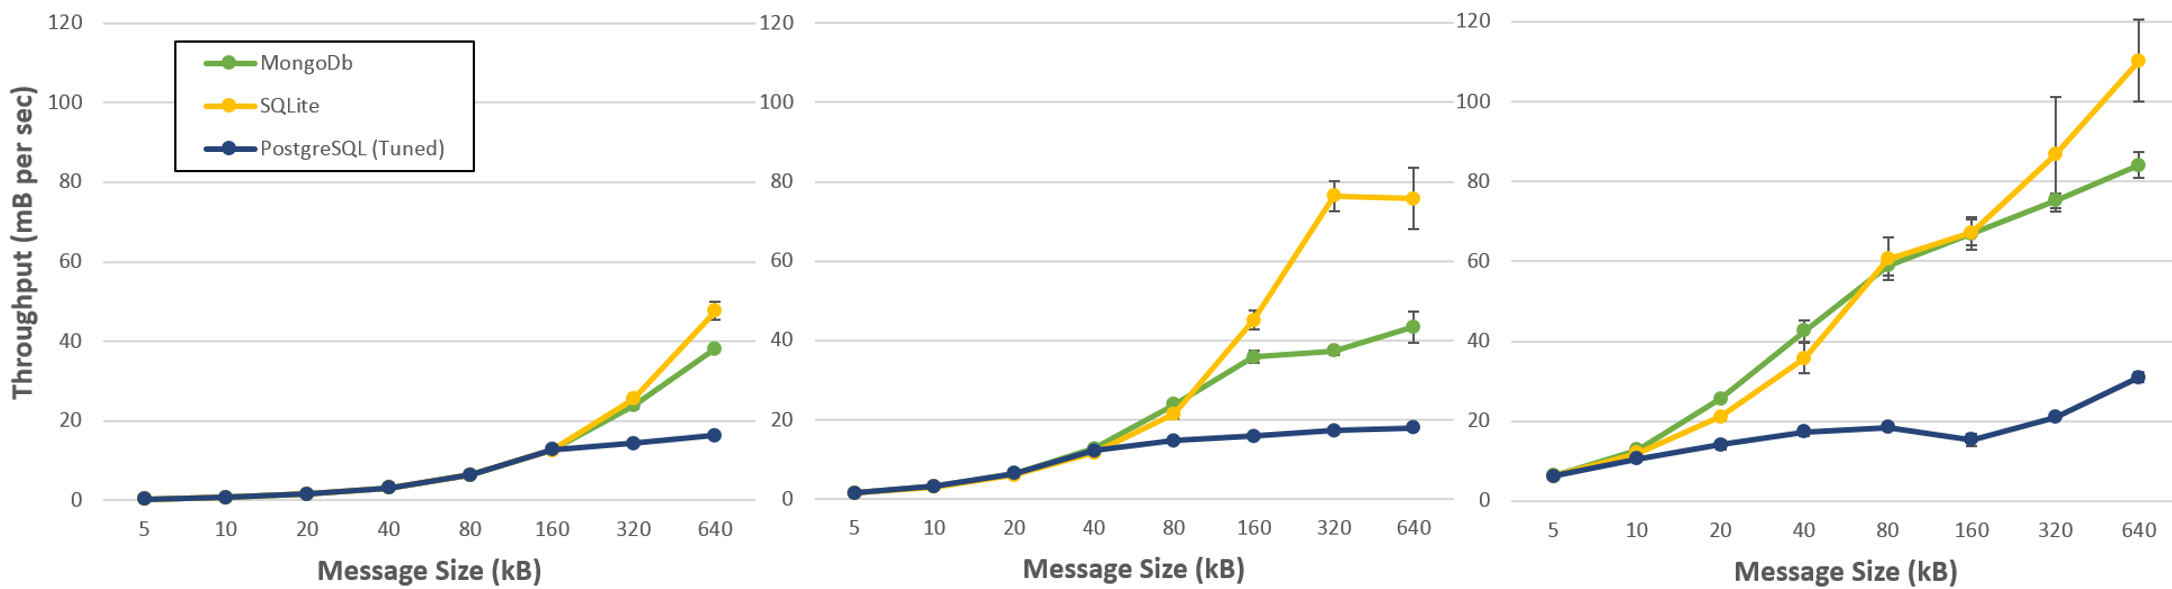
\includegraphics[width=\linewidth]{images/throughput}
    \subfloat[4 Messages Per Second]{%
        \hspace{0.3\linewidth}
        \label{4hz}%
    }
    \subfloat[16 Messages Per Second]{%
        \hspace{0.4\linewidth}
        \label{16hz}%
    }
    \subfloat[64 Messages Per Second]{%
        \hspace{0.3\linewidth}
        \label{64hz}%
    }
    \caption{Measurement of Throughput Across Multiple Frequencies and Message Sizes}
    \label{fig:throughput}
\end{figure*}

\subsection{Measuring Throughput}
\label{sec:throughput}
In the ROS ecosystem, published topics vary significantly in both the frequency at which messages are sent upon them, and in the size of messages belonging to the topic. This makes sense when considering that message types are very diverse, i.e. laser scans, joint angles, system events, etc. Therefore, in order to effectively compare the throughput of the three databases in consideration, several synthetic datasets were generated, reflecting potential types of messages that could appear in the ROS network. A constant 20 topics were generated for each synthetic data stream with each topic generating 500 messages. Additionally, each topic subscriber in the logging program was limited to an incoming message queue size of 10. This means that if messages are received by the logger faster than the underlying database can persist the messages, messages will be dropped from the incoming queue. This serves as a method of determining maximal throughput for each database. As frequencies and message sizes are increased, messages will begin to be dropped when the database has reached it maximum throughput for inserts corresponding to messages of the given size. Therefore, message sizes were varied on an exponential scale (each size is twice the previous message size) from 5000 bytes (approximately the size of a \textit{tf} message describing a coordinate frame transformation) to 0.64 Mb (approximately the size of a laser scan frame). To capture the effect of topic frequency on throughput, data streams were generated at three different frequencies: 4 hz, 16 hz, and 64 hz. Altogether, this resulted in the generation of 24 different data streams (3 frequencies by 8 message sizes). Each database was tested by logging each data stream 5 times in order to obtain reliable average throughput values over each stream. The experiment was run on a computer system running with an Intel Core i7-4770 CPU with 8 cores, 16 GB of memory, and a local hard disk.

\subsubsection{Tuning PostgreSQL}
In preliminary tests it was observed that PostgreSQL was performing significantly worse than both SQLite3 and MongoDB on the throughput experiment. It was determined that this was likely due to the fact that the our naive implementation of the PostgreSQL-ROS interface inserted each ROS message in autocommit mode. This means that each message was inserted in its own transaction. This clearly causes some amount of unnecessary overhead, although the degree to which using autocommit mode slows down PostgreSQL was unclear. Therefore, an additional test was run in which the naive PostgreSQL-ROS interface was re-engine-ered in order to allow message inserts to be batched into 2 second groups for each database transaction under the hypothesis that this optimization could yield significantly greater throughput values by decreasing overhead. As can be seen in Figure \ref{fig:throughput}, this optimization did yield improved throughput for the PostgreSQL database. To further tune the PostgreSQL engine, both the effective cache size and shared buffer size were increased to rather aggressive levels (12Gb and 4Gb respectively) in order to prevent encourage maximally efficient inserts. Again, this optimization improved overall PostgreSQL performance, but only by a small amount when considering the throughput values obtained by SQLite3 and MongoDb. Figure \ref{fig:throughput} references the throughput values for the final optimized version of the PostgreSQL engine determined in this section.

%; however, SQLite3 and MongoDB were still significantly better, often by factors of 2 to 3 times greater throughput.

\subsubsection{Results}
Results for the throughput evaluation against PostgreSQL, MongoDb, and SQLite3 can be seen in Figure \ref{fig:throughput}. Figure \ref{fig:throughput} splits these results into three graphs, one for each of the frequency levels. Interestingly, PostgreSQL performed significantly worse than both SQLite3 and MongoDb. 

It is important to note in Figure \ref{fig:throughput} that the points on the left of each graph at which all four implementations achieved that same throughput are points at which all messages made it into the database. These values therefore do not indicate a maximum throughput for the given message frequency and size. However, divergence of the throughput graphs at larger message sizes indicate that only some fraction of the total number of messages generated were actually inserted into the database, indicating the maximal throughput for each database at these given message frequencies and sizes. 

\hl{Explain the figure and why throughput increases with frequency and size: The general upward trend towards greater throughput for higher frequencies and for larger messages}

\subsubsection{Logging System Design Implications}

\hl{What are the salient points we can extract from these results? 1) For the scenario where we only have a single node available for the logging, SQLite3 performs the best due to its very low overhead, 2) in contrast, SQLite3 is not intended for distributed systems, so in the case where more than one machine is available for logging, the distribution-centric design of MongoDB in addition to its excellent throughput capabilities make it a good candidate for using in logging ROS messages.}

\subsection{Real World Performance}
\label{sec:realworld}
The previous section stress tested each of the databases by generating a fixed number of topics with messages of fixed sizes all sent at fixed frequencies. While this was a reasonable setup for measuring throughput, it is not necessarily representative of a real world work load. This is due to the fact that real world ROS networks contain many topics each with messages of different sizes and frequencies (see Figure \ref{fig:ros}). In order to evaluate how each of the databases performs on this type of real world dataset with significant variance among topics and messages, we tested the databases against several recordings from the MIT Stata Center dataset (labeled \textit{MIT1} and \textit{MIT2}). The MIT Stata Center dataset is a series of bagfiles consisting of recordings of image and laser data recorded at a high frequency by a robot exploring the Stata Center at MIT. This dataset is typically used for testing simultaneous localization and mapping algorithms and is therefore a set of recordings with very high rate of data flow. In order to test the real world performance of each database on a more moderate rate of data flow, several rosbag recordings obtained from previous research in our lab, were also tested against (labeled \textit{HCR1} and \textit{HCR2}). This series of tests used the same logging framework as in Section \ref{sec:throughput} (described in Figure \ref{fig:roslog}).

\begin{figure}
    \centering
    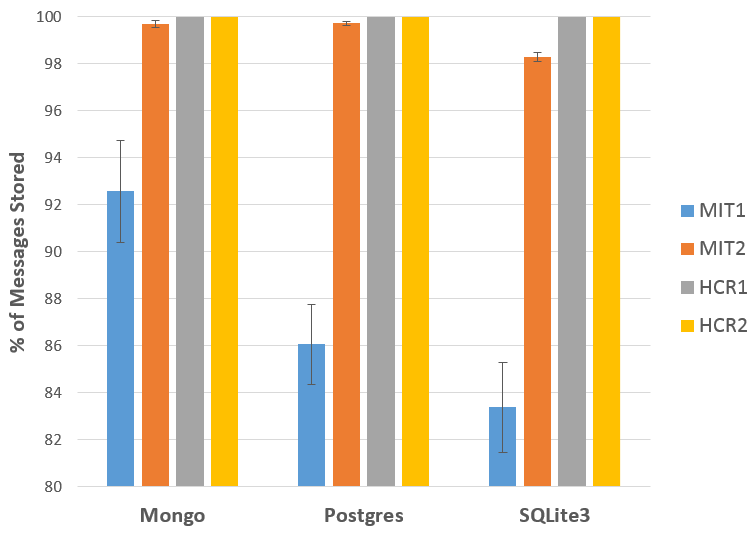
\includegraphics[width=\linewidth]{images/realworld}
    \caption{Percentage of Messages Persisted Across Four Real World Datasets. \textit{MIT1} and \textit{MIT2} are bagfiles from the MIT Stata center dataset and \textit{HCR1} and \textit{HCR2} are bagfiles from previous robotics experiments run in the Human-Centered Robotics Lab at the University of Washington. Note that the vertical axis shows the range (80, 100).}
    \label{fig:realworld}
\end{figure}

\subsubsection{Experiment dataset}
To evaluate how useful the logging system would be to a robotics researcher, we evaluated the time taken execute several representative queries for an experiment dataset (\textit{HCR1}).

% \subsection{Current State and Remainder of Project}
% Up to this point, the major set of work completed in this project has been in developing a multithreaded logging node for ROS, the database connectors which allow the logger to persist data to any of the given databases, and a testing framework for automating the throughput experiments in section \ref{sec:throughput}. Given this framework of code, the second study, in section \ref{sec:realworld}, is simply a matter of running the throughput automation script with the appropriate inputs specified (real world data set instead of the synthetic data set). Therefore, this portion should not be a major hurdle moving forward. The main issues remaining involve finishing the SQLite3 connector so that the throughput results for SQLite3 can be integrated into Figure \ref{fig:throughput}. Additionally, the portion of the study dealing with query performance still needs to be coded and tested. A majority of our efforts moving forward will be dedicated to this section.

% \subsubsection{Robotics Query Performance}
% We want to explore the expressivity of the query functionality for each database in addition to the time required to execute several representative queries over ROS message datasets. One set of queries we would like to test is retrieving messages based on values inside the messages. Clearly, any database system used for logging ROS messages will need to have the ability to query over JSON messages. Another set of queries to try is to retrieve a set of messages between two points in time. However, we are still considering what kinds of queries would be more interesting. This is challenging because ROS messages tend to represent readings from different sensors, which are not synchronized to produce messages at the same time. Therefore, it is hard to compute joins across different types of sensors. For example, one topic might receive a message whenever the robot's gripper is opened or closed, which occurs infrequently, while another topic might output the position of the robot's gripper in 3D space, which is output many times a second. An example of an interesting query would be to compute how much time is spent moving the robot's gripper while it is open. However, it's not clear how to write this query in any of the database systems we're evaluating. As a result, we may just evaluate how easy and efficient it is to query for data, such that we can manually compute the answers to more complex queries.

The research questions we wanted to answer from the dataset included the following queries:
\begin{enumerate}[label=Q\arabic*]
\item Get the number of times the right gripper was closed
\item Get the amount of time the camera was behind the robot
\item Get the number of times the right gripper was moved while in a particular region
\item Get the number of times a grasp was attempted with the right gripper when the camera was in front of the robot (+/- 0.1 seconds)
\end{enumerate}

The time for each query is shown in figure X.

\begin{figure}
\centering
\begin{tabular}{c | c | c | c | c}
  & Q1 & Q2 & Q3 & Q4 \\
 \hline
 MongoDB & & & & \\
 Postgres & & & & \\
 SQLite3 & & & & \\
 MongoDB (indexed) & & & & \\
 Postgres (indexed) & & & & 
\end{tabular}
\caption{Query times for each query using MongoDB, PostgreSQL, and SQLite3. For MongoDB and PostgreSQL, we also report query times after creating indices designed for each query.}
\label{fig:my_label}
\end{figure}

% Query:
% select sum(foo.count) from (select count(*) from r_gripper_controller__command where CAST(data::json->>'position' AS real)=0 union select count(*) from l_gripper_controller__command where CAST(data::json->>'position' AS real)=0) as foo;
% Result: 10

Complex queries: how to compute number of times the camera was moved, by counting number of runs of changing values.

MongoDB

% Add paragraph about lines of code necessary to answer these questions

% MongoDB
% Get the number of times the right gripper was closed
% db.r_gripper_controller__command.find({'position': 0.0}).count()
% 3
% millis: 0

% Get the amount of time where the camera was behind the robot.
% db.rviz_camera_publisher__camera_pose.find({'position.x': {$lte: 0}}).count()
% 1292
% millis: 22

% Get the number of times the right gripper was moved in a particular region
% db.r_cart__command_pose.find({
%   'pose.position.z': {$gt: 1},
%   'pose.position.y': {$gt: -0.5, $lt: 0.5},
%   'pose.position.x': {$gt: 0.5, $lt: 1}
% }).count()
% 618
% millis: 2

% Get the number of times a grasp was attempted with the right when the camera was in front of the robot (+/- 0.5 seconds)
% db.r_gripper_controller__command.find({'position': 0.0}).map(
%   function(evt) {
% 	  var evtTime = evt._meta.inserted_at.getTime();
%     var row = db.rviz_camera_publisher__camera_pose.findOne({
%       'position.x': {$gte: 0},
%       '_meta.inserted_at': {
% 			  $lt: new Date(evtTime + 500),
% 				$gt: new Date(evtTime - 500)
% 			}
%     })
% 		return row;
%   }
% ).length
% 3
% millis: 60


% SQLite3:
%
%   --Q1
%       SELECT COUNT(*) as count
%       FROM r_gripper_controller__command 
%       WHERE json_eq_field(msg, position, 0);
%
%       result: 3, 0.29ms (25.54ms on second run)
%
%   --Q2
%       SELECT COUNT(*) 
%       FROM rviz_camera_publisher__camera_pose
%       WHERE json_le_field(msg, 'position.x', 0);
%
%       result: 1292, 138.73ms (20886.92ms on first run)
%
%   --Q3
%       SELECT COUNT(*) 
%       FROM r_cart__command_pose
%       WHERE json_gt_field(msg, pose.position.z, 1)
%       AND   json_gt_field(msg, pose.position.y, -0.5)
%       AND   json_lt_field(msg, pose.position.y, 0.5)
%       AND   json_gt_field(msg, pose.position.x, 0.5)
%       AND   json_lt_field(msg, pose.position.x, 1);
%
%       result: 618, 80.14ms (4645.94ms on first run)
%
%   --Q4
%       



%\section{Discussion}


%\section{Conclusion}


\bibliographystyle{abbrv}
\bibliography{references.bib}  

%\balancecolumns

\end{document}

